\chapter{Reti neurali}
\label{Capitolo 4}
%%%%%%%%%%%%%%%%%%%%%%%%%%%%%%%%%%%%%%%%%%%%55
%%%%%%%%%%%%%%%%%%%%%%%%%%%%%%%%5

In natura l'operazione di \textit{learning} viene eseguita tramite il
\textbf{cervello}, che tramite i \textbf{neuroni}, delle cellule nervose, è in
grado di effettuare una miriade di operazioni in parallelo. Potenzialmente i
neuroni hanno un tempo di risposta nell'ordine dei millisecondi mentre in
circuito logico si aggira nell'ordine dei nanosecondi quindi la differenza deve
essere ricercata nell'\textit{architettura} del nostro cervello. La ``potenza di
calcolo'' del cervello è data dal funzionamento parallelo di $\sim 10^{11}$
neuroni, collegati tra loro da $\sim 10^5$ connessioni. Vediamo quindi
indicativamente gli elementi principali di un \textbf{neurone biologico}:
\begin{itemize}
	\item \textbf{corpo}, che implementa tutte le funzioni logiche del neurone
	\item \textbf{assone}, il canale di uscita verso gli altri neuroni, è quello
	      che si occupa di trasmettere gli impulsi nervosi
	\item \textbf{dendrite}, la parte che permette al neurone di ricevere gli
	      impulsi nervosi
	\item \textbf{sinapsi}, ovvero la regione funzionale in cui avviene lo scambio
	      dei segnali, ovvero dove ogni singolo ramo terminale dell'assone
	      (\textbf{bottone sinaptico}) del neurone (detto \textbf{neurone
	      pre-sinaptico}) trasmette impulsi nervosi provenienti dal neurone ai
	      dendriti di altri neuroni (detti \textbf{neuroni post-sinaptici})
\end{itemize}
Questa ``architettura'' è quindi basata sull'emissione di segnali da parte del
neurone. Questa azione dipende da vari fattori, come ad esempio la forza del
segnale ricevuto da altri neuroni e la forza delle connessioni di un neurone con
le sue sinapsi. Si ha che la \textbf{funzione di risposta} di un neurone è una
funzione non lineare impulso ricevuto dai dendriti. Dopo l'invio di un impulso
ogni neurone ha un tempo, detto \textbf{refractory time}, prima del quale poter
inviare un altro impulso. Si hanno infatti due stati possibili per il
\textit{neurone biologico}:
\begin{enumerate}
	\item \textbf{eccitazione}, quando il neurone invia, tramite le sinapsi,
	      segnali (che per comodità computazionale chiamiamo già \textbf{pesati}) ai
	      neuroni connessi
	\item \textbf{inibizione}, quando il neurone non invia segnali
\end{enumerate}
La \textbf{transizione di stato} dipende dall'entità complessiva dei segnali
eccitatori e inibitori ricevuti dal neurone.\\
Una legge importante è la \textbf{regola di Hebb} che indica che i cambiamenti
di forza delle connessioni delle sinapsi di due neuroni connessi è proporzionale
alla correlazione tra l'emissione di segnali dei neuroni stessi (ovvero se due
neuroni rispondono allo stesso input allora è bene che siano connessi).
\section{Unità di calcolo nelle reti neurali}
Lo studio di un singolo neurone non è comunque particolarmente interessante. Si
introduce quindi lo studio di \textbf{reti neurali} dove vengono posti diversi
\textit{neuroni} in modo che possano fare qualcosa di utile.\\
Se dal singolo neurone voglio passare alla rete collego in modo orientato i
neuroni, di modo che l'output di uno sia l'input dell'altro. \\
Si hanno alcune \textbf{caratteristiche strutturali} delle \textit{reti neurali
artificiali}:
\begin{itemize}
	\item hanno un gran numero di unità
	\item permettono operazioni elementari
	\item hanno un alto livello d'interconnessione
\end{itemize}
Ci sono anche alcune \textbf{caratteristiche dinamiche}:
\begin{itemize}
	\item si hanno cambiamenti di stato in funzione dello stato dei neuroni
	      collegati in input
	\item si ha una funzione di uscita per ogni unità
	\item si ha la modifica dello schema di connessione, tramite la modifica dei
	      pesi, per l'apprendimento
\end{itemize}
Dal punto di vista formale, dovendo espandere le definizioni fatte nel caso del
singolo neurone a più neuroni, si lavora con:
\begin{itemize}
	\item una \textbf{matrice dei pesi} $W$, con i valori indicati tramite
	      $w_{ij}$, per gli archi che collegano i neuroni. I pesi sono i \textit{pesi
	      correnti} (un vettore di pesi per ogni neurone e quindi una matrice, che
	      risulta a singolo colonna se ho un solo neurone)
	\item un \textbf{vettore delle soglie} $\Theta$, con i valori indicati tramite
	      $\theta_i$, una per ogni neurone
	\item l'\textbf{input netto per il neurone $i$ al tempo $t$}, indicato con\\
	      $n_i(t)=\sum_{j=1}^n w_{ij}\cdot s_j(t)-\theta_i$, quindi si ha che la soglia
	      influisce già nell'input del neurone (e quindi non si può ragionare come se
	      $\theta$ fosse un confronto a posteriori)
	\item la \textbf{funzione di transizione} indicata con $s_i(t+1)=g(n_i(t))$
\end{itemize}
L'output di un neurone è, a conti fatti, uno stato per un altro neurone.\\
Si hanno alcuni elementi caratterizzanti di una rete neurale:
\begin{itemize}
	\item il \textbf{tipo di unità}
	\item la \textbf{topologia}, ovvero la direzione delle connessioni
	      (\textit{feedforward \textnormal{o} feedback}), il numero di neuroni (con più
	      layer o solo uno, \textit{monostrato \textnormal{o} multistrato}) etc$\ldots$
	\item le \textbf{modalità di attivazione}, che può essere \textit{seriale
		ciclica, seriale probabilistica, parallela \textnormal{o} mista}
	\item un \textbf{algoritmo di apprendimento} con lo studio, in primis, dei
	      pesi
\end{itemize}
\newpage

Quindi le reti neurali sono composte da nodi o \textbf{unità} unite da \textbf{collegamenti} diretti. Un collegamento dall'unità $j$ all'unità $i$ serve a propagare l'attivazione $a_j$ da $j$ a $i$. A ogni collegamento è associato il \textbf{peso} $W_{j,i}$ che determina quindi la forza e il segno della connessione. La figura \ref{Neurone} ne mostra un esempio. 
\begin{figure}[h!]
	\centering
	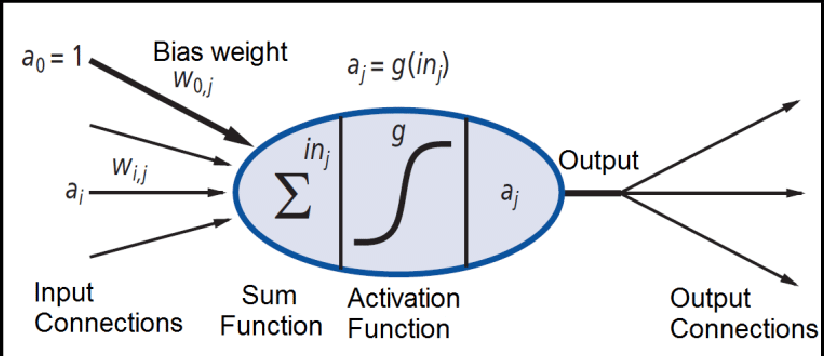
\includegraphics[width=0.75\textwidth]{img/An-artificial-neuron-and-its-various-components-Adapted-from-Norvig-Russel-2013-p.png}
	\caption{Neurone Artificiale}
	\label{Neurone}
\end{figure}
Ogni unità $i$ calcola per prima cosa una somma pesata dei propri input:
\[in_i=\sum_{j=0}^n W_{j,i}\cdot a_j\]
Fatto questo, applica una \textbf{funzione di attivazione} $g$ alla somma per derivare l'output:
\[a_i=g(in_i)=g(\sum_{j=0}^n W_{j,i}\cdot a_j)\]
La funzione di attivazione $g$ è progettata per soddisfare due requisiti:
\begin{itemize}
	\item Prima di tutto desideriamo che l'unità sia attiva (vicina ad 1) quando sono dati i valori giusti di input, altrimenti vogliamo che essa sia inattiva (vicina a -1).
	\item L'attivazione deve essere non lineare.
\end{itemize}Per definire i \textbf{due stati del neurone} si usa l'insieme $\{0, 1\}$ o l'insieme $\{-1, 1\}$ (si ha infatti un \textbf{neurone binario}). La \textbf{funzione di transizione} viene indicata con:
\[s(t+1)=1 \mbox{\textnormal{sse} }\sum w_i\cdot s_i(t)\geq \theta\]
ovvero in un tempo successivo $t+1$ (con $s(t)$ che definisce uno stato al tempo
$t$) ho che il neurone emette il segnale (stato

pari ad 1) sse al tempo precedente $t$ ho avuto una somma pesata, tramite $w_i$,
degli input $a_i(t)$ maggiore della soglia
$\theta$.\\
La funzione di attivazione $g$ può essere rappresentata da diverse funzioni, tra cui:
\begin{itemize}
	\item La funzione Soglia
	\item La funzione Sigmoide/Logistica
\end{itemize}
\begin{figure}[h!]
	\centering
	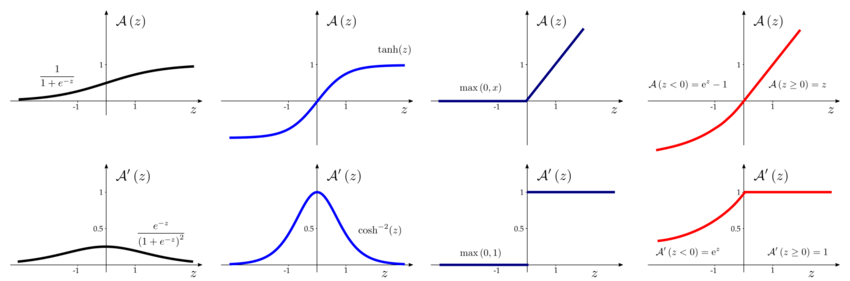
\includegraphics[width=1\textwidth]{img/Some-of-the-most-common-activation-functions-and-their-first-order-gradient-From-left-to.png}
	\caption{Funzioni di Attivazione}
	\label{ActivationFunction}
\end{figure}
L'insieme degli stati, rappresentato in modo binario, comporta che la funzione
di transizione sia una \textbf{funzione soglia}:
\[g(\sum_{j=0}^n W_{j,i}\cdot a_j)=
	\begin{cases}
		1 & \mbox{se } \sum_{j=0}^n W_{j,i}\cdot a_j\geq \theta \\
		0 & \mbox{altrimenti}                                   
	\end{cases}
\]
Questo modello è comunque estremamente semplificato. L'insieme degli stati
potrebbe non essere booleano ma potrebbe essere $\mathbb{R}$, infatti anche
nella biologia il segnale in uscita dai neuroni è graduato e continuo. Si
potrebbe quindi avere una \textbf{funzione logistica o sigmoide}, dove, avendo
come insieme degli stati $\mathbb{R}$ si avrebbe:
\[f(x)=\frac{1}{1+e^{-x}}\,\,\,\,\mbox{  con } \,\,\, x=\sum w_i\cdot a_i\]
Il peso di \textbf{bias} indicato da $W_{0,j}$ determina la soglia effettiva dell'unità e sarebbe uguale a quello che è indicato da $\theta$.
\begin{definizione}
	Se una rete possiede $s_j$ unità nel layer $j$ e $s_{j+1}$ nel layer $j+1$, allora $W$ avrà dimensioni pari a $s_j+1 \times (s_j + 1)$.
\end{definizione}
L'output della rete può essere simboleggiato in diversi modi, solitamente i diversi testi si accordano su una delle seguenti nomenclature: $y, h_\theta(x), h_w(x)$. Quindi non bisogna confondersi qualora in un esempio comparisse $h_\theta(x)$ al posto di $h_w(x)$.
\section{Struttura della rete}
Ci sono due categorie principali di strutture di reti neurali:
\begin{itemize}
	\item Feed-Forward / Alimentata in avanti
	\item Ricorrenti
\end{itemize}
Questo libro si concentrerà sulle strutture \textbf{Feed-Forward}. Esse sono abitualmente organizzare in \textbf{strati}, in modo tale che ogni unità riceva in input solo dalle unità nello strato immediatamente precedente. Oltretutto esse permettono anche la possibilità di avere degli strati nascosti e, di conseguenza, delle unità nascoste. In questa sezione introdurremo due tipologie di reti neurali:
\begin{itemize}
	\item Single Layer: 
	      Nelle reti neurali a \textbf{single layer} un insieme d'input è direttamente mappato su un layer di output. Questa semplice istanziazione di rete è anche chiamata come \textit{percettrone}.
	\item Multi Layer: dove il layer d'input e quello di output sono separati da un gruppo di \textbf{layer nascosti}. 
\end{itemize}
Solitamente nell'\textbf{input layer} i nodi in input vengono descritti da un \textbf{vettore} $X = a_0$.
\subsection{Reti neurali a uno strato alimentate in avanti: il percettrone}
Questa tipologia di architettura possiede un singolo \textbf{input layer} e un \textbf{output layer}. La figura \ref{Percettrone} mostra un esempio della struttura.
\begin{figure}[h]
	\centering
	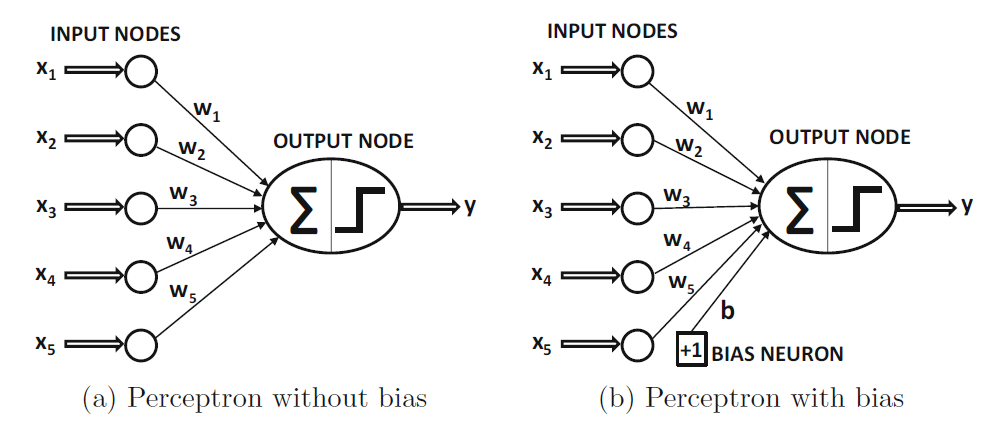
\includegraphics[width=1\textwidth]{img/Capture.PNG}
	\caption{Percettrone}
	\label{Percettrone}
\end{figure}
\begin{definizione}
	Un percettrone è una collezione di neuroni, di cardinalità $M$, a cui viene
	aggiunto un insieme di nodi in input, di cardinalità $N$ (generalmente
	diversa da quella della collezione di neuroni). Generalmente gli input sono
	pesati e con la notazione $w_{ij}$ indichiamo il peso della connessione tra il
	nodo $i$-simo in input e il neurone $j$-simo.\\
	I neuroni sono tra loro completamente indipendenti comportando anche un
	insieme di elementi in output. Nel caso semplice di funzioni di transizione
	binarie l'output sarà quindi un vettore binario contenente all'indice $k$-simo
	1 se il neurone $k$ ha inviato il segnale o 0 altrimenti. \\
	Solitamente coi percettroni si parla di \textit{learning supervisionato}.
\end{definizione}
Sappiamo che un percettrone a \textbf{soglia} restituisce 1 se e solo se la somma pesata dei suoi input (bias incluso) è positiva:
\[\sum_{j=0}^n W_j\cdot x_j > 0\]\,\,\,\mbox{oppure}\,\,\,\[W\cdot x > 0\]
Dal punto di vista geometrico l'equazione $W\cdot x$ rappresenta un 
\textbf{iperpiano} nello spazio d'input (che è una retta in $\mathbb{R}^2$) che separa i possibili
vettori d'input in due classi, a seconda che formino con $W$ un angolo acuto o
ottuso. Quindi il percettrone restituisce $1$ se e solo se l'input si trova da una parte specifica rispetto a tale iperpiano. Per questa ragione, il percettrone a soglia è chiamato anche \textbf{separatore lineare}. Difatti esso può rappresentare \textbf{funzioni linearmente separabili} (fig. \ref{SeparatoreLineare}).\\
\begin{figure}[h!]
	\centering
	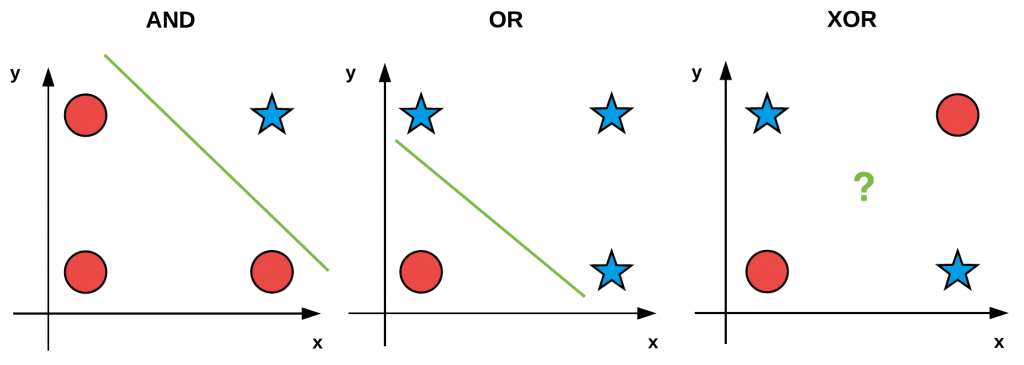
\includegraphics[width=1\textwidth]{bitwise_datasets-1024x365.png}
	\caption{Separatore Lineare}
	\label{SeparatoreLineare}
\end{figure}
È chiaro quindi che i \textbf{percettroni a soglia possono rappresentare solo funzioni linearmente separabili}. D'altro Canto esiste un semplice algoritmo di apprendimento capace di adattare un percettrone a soglia a qualsiasi insieme di addestramento linearmente separabile.
\subsubsection{Algoritmo del percettrone e Discesa del Gradiente}
Fino a ora il singolo neurone rappresentava un singolo iperpiano che veniva ``spostato'' per dividere le istanze positive e quelle negative. Ora introduciamo che a ogni passo di aggiornamento si aggiornano i pesi e se, mano a mano che cambio i pesi, misuro l'errore sul dataset del mio sistema. Si può quindi far ``scendere'' questo errore e ci si augura che ci sia una costante di discesa dell'errore. L'idea di questo algoritmo è di calibrare i pesi nella rete in modo da minimizzare una qualche misura di errore sull'insieme di training. Quindi L'apprendimento è formulato come una ricerca di ottimizzazione nello \textbf{spazio dei pesi}. La misura di errore è la \textbf{somma dei quadrati degli errori}.
Il quadrato dell'errore per un singolo esempio di training con input $x$ e output $y$ si scrive:
\[E=\frac{1}{2}(y-h_w(x))^2\]\mbox{Dove $h_w(x)$ è l'output del percettrone per l'esempio.}

Possiamo usare il \textbf{metodo della discesa di gradiente} per ridurre il quadrato dell'errore calcolando la derivata parziale di $E$ rispetto a ogni peso. Nell'algoritmo a discesa del gradiente, in cui vogliamo \textbf{ridurre} E, aggiorniamo i pesi come segue:
\[w_{ij}\gets w_{ij}+\eta\cdot(y-h_w(x))\times a_i\]
Si calcola il gradiente della curva degli errori e si punta a essere sempre in ``discesa'' lungo la curva dell'errore, aggiustando in modo opportuno i pesi. Viene anche introdotto il \textbf{learning rate (\textit{tasso di apprendimento})} $\eta$, utile per stabilire la velocità di apprendimento della rete. In pratica $\eta$ decide quanto cambiare il peso (e se si vuole trascurare il parametro basta porre $\eta =1$). L'uso di tale parametro migliora la stabilità della \textit{rete neurale} che non avrà cambi di peso eccessivi, anche se
questo comporta tempi di apprendimento più estesi. Tipicamente si ha che:
\[0.1\leq\eta\leq 0.4\]
Si noti che se l'errore $y-h_w(x)$ è positivo allora $y>h_w(x)$ quindi l'output della rete dev'essere troppo piccolo e quindi i pesi aumentano per gli input positivi e diminuiscono per quelli negativi. Quando l'errore è negativo avviene l'opposto. Gli esempi di addestramento vengono fatti passare attraverso la rete uno per volta, modificando leggermente i pesi a ogni iterazione per ridurre l'errore. Ogni ciclo attraverso tutto gli esempi prende il nome di \textbf{epoca}. Le epoche sono tipicamente ripetute fino a quando non viene soddisfatto qualche criterio di terminazione. Si ha che a ogni iterazione ci si aspetta un miglioramento della \textit{rete neurale} (e questo miglioramento è dimostrabile). Viene imposto
quindi un limite $T$ d'iterazioni entro le quali interrompere l'apprendimento anche se non si è arrivati al risultato
corretto.
% \begin{algorithm}[h] % TODO: modify
% 	\begin{algorithmic}
% 		\Function{grad}{}
% 		\State \textit{inizializzo ogni $\Delta w_i$ a $0$}
% 		\For {\textit{ogni input $\langle( x_1, \ldots x_n), t\rangle$}}
% 		\State \textit{invio l'input $( x_1, \ldots x_n)$ all'unità lineare e
% 		calcola l'output $y$} 
% 		\State \textit{aggiorno la variazione dei pesi:}
% 		\[\Delta w_i=\Delta w_i+\eta\cdot (t-y)\cdot x_i\]
% 		\EndFor
% 		\State \textit{aggiorno i pesi:}
% 		\[w_i=w_i+\Delta w_i\]
% 		\EndFunction
% 	\end{algorithmic}
% 	\caption{Algoritmo di discesa lungo il gradiente}
% \end{algorithm}
% Abbiamo una \textbf{modalità Batch}, quindi computazionalmente costosa:
% \[w=w-\eta\cdot\nabla E_D[W]\]
% Si può avere una \textbf{modalità incrementale}:
% \[w=w-\eta\cdot\nabla E_d[W]\]
% calcolata sui singoli esempi $d$:
% \[E_d[w]=\frac{1}{2}(t_d-y_d)^2\]
% La discesa lungo il gradiente incrementale può approssimare la discesa lungo
% il gradiente Batch arbitrariamente se $\eta$ è abbastanza piccolo.\\
% Rispetto a quanto visto per il percettrone la discesa lungo il gradiente
% converge all'ipotesi con il minimo errore quadratico se  $\eta$ è abbastanza
% basso, anche per dati di training molto rumorosi.

% \[\Delta w_{ik}=-(y_k-t_k)\times a_i\]
% In questo discorso bisogna inserire anche la soglia, importante per input
% specifici (basti pensare a un input pari a 0 che annullerebbe ogni cambio di
% peso secondo la formula precedente). Per ora trascureremo tali casi anche se una
% semplice soluzione per un caso limite come quello di avere solo input nulli, è
% quella di aggiungere un \textbf{nodo bias}, di valore $-1$, collegato ai neuroni
% con peso nullo.\\


\subsubsection{Approfondimento sul Percettrone}
Vediamo due teoremi utili per lo studio dell'apprendimento del percettrone su due classi $A$ e $B$, banalmente rappresentanti, nella nostra situazione binaria e semplificata, il caso in cui si abbia il neurone che emette il segnale (valore 1 in output) o altrimenti (valore 0 in output). Nel nostro caso le classi sono discriminabili.
\begin{definizione}[definizione di convergenza]
	Comunque si scelgano i pesi iniziali, se le classi A e B sono discriminabili,
	la procedura di apprendimento termina dopo un numero finito di passi
\end{definizione}
\begin{definizione}[definizione di Minsky e Papert]
	La classe delle forme discriminabili da un percettrone semplice è
	limitata alle forme linearmente separabili
\end{definizione}
In base a questo si distinguerà in:
\begin{itemize}
	\item \textbf{addestramento separabile}, quando si ha un iperpiano che separa
	      le istanze positive e negative
	\item \textbf{addestramento non separabile}
\end{itemize}
Per capire il discorso della \textbf{separabilità} vediamo un esempio.
\begin{esempio}
	Vediamo un esempio che tratta l'addizione binaria, ovvero l'\textit{or
	esclusivo}.
	Le possibili istanze sono rappresentate nel piano:
	\begin{figure}[H]
		\centering
		\psscalebox{1.0 1.0} % Change this value to rescale the drawing.
		{
			\begin{pspicture}(0,-1.9534792)(5.906958, 1.9534792)
				\psline[linecolor=black, linewidth=0.04,
					arrowsize=0.05291667cm 2.0, arrowlength=1.4
				, arrowinset=0.0]{->}(2.4,-1.9534792)(2.4, 1.6465209)(2.4, 2.046521)
				\psline[linecolor=black, linewidth=0.04,
					arrowsize=0.05291667cm 2.0, arrowlength=1.4,
				arrowinset=0.0]{->}(1.6,-1.1534791)(6.0,-1.1534791)
				\psdots[linecolor=black, dotsize=0.4](2.4, 0.84652084)
				\psdots[linecolor=black, dotsize=0.4](4.4, 0.84652084)
				\psdots[linecolor=black, dotsize=0.4](4.4,-1.1534791)
				\psdots[linecolor=black, dotsize=0.4](2.4,-1.1534791)
				\rput[bl](0.4, 0.68652084){$0\oplus 1=1$}
				\rput[bl](0.4,-0.7534792){$0\oplus  1=0$}
				\rput[bl](3.4,-0.7534792){$1\oplus 0=1$}
				\rput[bl](3.4, 1.2465209){$1\oplus 1=0$}
			\end{pspicture}
		}
	\end{figure}
	Ho quindi che nessuna retta potrà separare tutti i punti e
	quindi i punti a valore 1 \textbf{non sono linearmente separabili} da quelli a
	valore 0.\\
	Si vorrebbe cercare un neurone binario a soglia tale che:
	\[x\oplus y=1\iff \alpha\cdot x+\beta\cdot y\geq \lambda\]
	Tale neurone si rappresenterebbe con:
	\begin{figure}[H] 
		\centering
		\psscalebox{1.0 1.0} % Change this value to rescale the drawing.
		{
			\begin{pspicture}(0,-1.9534792)(5.906958, 1.9534792)
				\pscircle[linecolor=black, linewidth=0.04,
				dimen=outer](3.2, 0.24245118){0.8}
				\psline[linecolor=black, linewidth=0.04,
					arrowsize=0.05291667cm 2.0, arrowlength=1.4,
				arrowinset=0.0]{->}(0.4, 0.64245117)(2.4, 0.64245117)
				\psline[linecolor=black, linewidth=0.04, arrowsize=0.05291667cm 2.0,
				arrowlength=1.4, arrowinset=0.0]{->}(0.4,-0.15754883)(2.4,-0.15754883)
				\psline[linecolor=black, linewidth=0.04, arrowsize=0.05291667cm 2.0,
				arrowlength=1.4, arrowinset=0.0]{->}(4.0, 0.24245118)(6.0, 0.24245118)
				\rput[bl](0.0, 0.56245117){$x$}
				\rput[bl](0.0,-0.32754883){$y$}
				\rput[bl](1.2, 0.8245117){$\alpha$}
				\rput[bl](1.2, 0.024245118){$\beta$}
				\rput[bl](3.07, 0.115754886){$\lambda$}
				\rput[bl](6.2, 0.0824245118){$x\oplus y$}
			\end{pspicture}
		}
	\end{figure}
	ma appunto tale neurone non può esistere in quanto non potrei mai separare
	i punti a valori 1 e quelli a valore 0 con una retta. Posso infatti separare o
	singoli punti o coppie di punti a valore opposto o triple di punti ma non
	potrò mai avere separati insiemi con tutti gli 0 e tutti gli 1.
\end{esempio}
\begin{definizione}
	Se l'insieme degli input estesi è partito in due classi linearmente separabili
	allora:
	\[\exists\,\, W\mbox{t.c }
		\begin{cases}
			1 & \mbox{se } \sum w_i\cdot a_i \geq 0 \\
			0 & \mbox{se } \sum w_i\cdot a_i < 0    
		\end{cases}
	\]
	con $W$ \textbf{vettore dei pesi}.
\end{definizione}
Vediamo quindi l'algoritmo di learning per un percettrone, data la
\textbf{funzione di transizione} per un input di cardinalità $m$ e $n$ neuroni:
\[
	y_j=g\left(\sum_{i=0}^m w_{ij}\cdot a_i \right)=
	\begin{cases}
		1 & \mbox{se } \sum_{i=0}^m w_{ij}\cdot a_i > 0    \\
		0 & \mbox{se } \sum_{i=0}^m w_{ij}\cdot a_i \leq 0 
	\end{cases}
\]
Vediamo quindi l'algoritmo di apprendimento del percettrone:
\begin{algorithm}[H]
	\begin{algorithmic}
		\Function{perceptron-learning}{}
		\State \textit{\color{gray}{\# Inizializzazione}}
		\State \textit{si imposta tutti i pesi $w_{ij}$ a valori casuali piccoli
		(anche negativi)}
		\State \textit{\color{gray}{\# Training}}
		\For {\textit{$T$ iterazioni \textbf{o} fino a che tutti gli output non sono
		corretti}}
		\For {\textit{ogni vettore input}}
		\State \small{\color{gray}{\textit{\# calcolo l'attivazione di ogni neurone
		$j$ }}}
		\State \small{\color{gray}{\textit{\# tramite la funzione di transizione
		$g$:}}} 
		\State $y_j=g\left(\sum_{i=0}^m w_{ij}\cdot a_i \right)=
		\begin{cases} 1
			  & \mbox{se } \sum_{i=0}^m w_{ij}\cdot a_i > 0 \\ 0 &\mbox{se }
			\sum_{i=0}^m w_{ij}\cdot a_i \leq 0
		\end{cases}$ 
		\State {\textit{\color{gray}\# aggiorno ogni peso individualmente}}
		\State {\textit{\color{gray}\# nella prossima iterazione avrò nuovi pesi}}
		\State $w_{ij}\gets w_{ij}-\eta\cdot(y_j-t_j)\times a_i$
		\EndFor
		\EndFor
		\State {\textit{\color{gray}\# Recall}}
		\State \small{\color{gray}{\textit{\# ricalcolo l'attivazione di ogni
		neurone $j$ tramite:}}} 
		\State $y_j=g\left(\sum_{i=0}^m w_{ij}\cdot a_i \right)=
		\begin{cases} 1
			  & \mbox{se } w_{ij}\cdot a_i > 0 \\ 0 &\mbox{se }
			w_{ij}\cdot a_i \leq 0
		\end{cases}$
		\EndFunction
	\end{algorithmic}
	\caption{Algoritmo di learning del percettrone}
\end{algorithm}
La complessità dell'algoritmo è $O(Tnm)$.\\
Si può dimostrare, tramite il \textbf{definizione della convergenza del percettrone}
che dopo $\beta$ modifiche di peso il percettrone classifica 
correttamente ogni input anche se tale $\beta$ non è il reale numero di stadi e
dipende dall'output.\\
L'algoritmo di apprendimento del percettrone quindi \textit{converge} alla
classificazione corretta quindi se:
\begin{itemize}
	\item i dati di training sono linearmente separabili
	\item $\eta$ è abbastanza piccolo
\end{itemize}
\begin{definizione}
	Se l'insieme degli input estesi è partito in due classi linearmente separabili
	$A$ e $B$ allora é possibile trovare un vettore di pesi $w$ tale che:
	\[
		\begin{cases}
			\langle w, x\rangle\geq 0 & \mbox{se }x\in A \\
			\langle w, x\rangle < 0   & \mbox{se }x\in B 
		\end{cases}
	\]
	Quindi:
	\begin{itemize}
		\item si parte con $w$ arbitrario
		\item si classifica un punto $x$:
		      \begin{itemize}
		      	\item se la risposta è corretta si ha $w'\gets w$
		      	\item se la risposta è errata:
		      	      \[
		      	      	\begin{cases}
		      	      		w'\gets w+x & \mbox{se }x\in A \\
		      	      		w'\gets w-x & \mbox{se }x\in B \\
		      	      	\end{cases}
		      	      \]
		      \end{itemize}
	\end{itemize}
	
\end{definizione}
\begin{proof}
	Vediamo la prova della correttezza del definizione.\\
	Se si ha $x\in A$ allora si ha $\langle w, x\rangle<0$ infatti, poiché:
	\[\langle x, x\rangle\geq 0\]
	si ha che:
	\[\langle w', x\rangle=\langle (w+x), x\rangle=\langle w, x\rangle+\langle x,
		x\rangle>\langle w, x\rangle\]
		Quindi $w'$ classifica $x$ in modo più corretto di $w$ anche se altri input
		possono essere classificati "meno correttamente".
		\end{proof}
		\begin{proof}
			Passiamo ora alla convergenza.\\
			Consideriamo quindi $A'=A\cup B'$ con:
			\[B'=\{-x|\, x\in B\}\]
			e cerchiamo un $v$ tale che:
			\[\langle v, x\rangle\geq 0,\,\,\forall\, x\in A'\]
			Si hanno quindi:
			\begin{itemize}
				\item la \textbf{sequenza di addestramento} $\{x_i\}_{i\in N}$ dove $x_i\in
				      A'$ e quindi la sequenza ontiene infiniti elementi sia di $A$ che di $B'$
				\item la \textbf{sequenza di pesi} $\{w_i\}_{i\in N}$ dove si parte
				      arbitrariamente con $w_0=0$ e si procede con:
				      \[
				      	\begin{cases}
				      		w_{k+1}\gets w_k     & \mbox{se }\langle w_k, x_k\rangle\geq 0 \\
				      		w_{k+1}\gets w_k+x_k & \mbox{altrimenti}                       
				      	\end{cases}
				      \]
			\end{itemize}
			Si hanno quindi:
			\begin{itemize}
				\item la \textbf{sequenza di pesi modificata} $\{v_i\}_{i\in N}$ 
				\item la \textbf{sottosequenza di training corrispondente} $\{v_i\}_{i\in N}$ 
			\end{itemize}
			Di modo che le coppie $(v_i, t_i)$ corrispondano ai $w_j$ tali per cui $w_j\neq
			w_{j+1}$.\\
			Ad esempio per:
			\[w_0\neq w_1=w_2=w_3\neq w_4=w_5=w_6\neq w_7\neq w_8\cdots\]
			avremo:
			\begin{itemize}
				\item $(v_0, t_0)$ associati a $w_0$
				\item $(v_1, t_1)$ associati a $w_3$
				\item $(v_2, t_2)$ associati a $w_6$
				\item $(v_3, t_3)$ associati a $w_7$
			\end{itemize}
			Avendo:
			\[\langle v_i, t_i\rangle<0\,\,\,\forall i\]
			e avendo:
			\[v_{i+1}=v_i+t_i=v_{i-1}+t_{i-1}+y_i=\sum_{k=0}^i t_i\]
			e quindi la sequenza $\{v_i\}$ è \textbf{finita}.
		\end{proof}
		\begin{proof}
			Uniamo matematicamente in una sola dimostrazione.\\
			Sia $w$ una qualsiasi soluzioni che sappiamo esistere per ipotesi. Si ha che:
			\[\langle v, x\rangle\geq 0,\,\,\forall\, x\in A'\]
			Pongo quindi:
			\[\alpha=\min(\langle x, w\rangle,\,\,\forall\, x\in A')\]
			sapendo che:
			\[v_{i+1}=v_i+t_i=v_{i-1}+t_{i-1}+y_i=\sum_{k=0}^it_i\]
			ho che:
			\[\langle v_{i+1}, w\rangle=\langle \left(\sum_{k=0}^i t_k \right),
				w\rangle\geq (i+1)\cdot\alpha\]
				ma usando il definizione di \textbf{Cauchy-Schwarz} si ha che:
				\[(\langle v_{i+1}, w\rangle)^2\leq \langle |v_{i+1}|^2,|w|^2\rangle\]
				ottenendo che:
				\[|v_{i+1}|^2\geq \frac{(i+1)^2\cdot \alpha^2}{|w|^2}\]
				Pongo quindi:
				\[M=\max\{|x|^2|,\, x\in A'\}\]
				si ha che, avendo $\langle v_{1}, t_i\rangle<0$:
				\[|v_{i+1}|^2=|v_i+t_i|^2=|v_i|^2+2\cdot\langle v_{i}, t_i\rangle+|t_i|^2\leq
					|v_i|^2+|t_i|^2\]
					Si ha, di conseguenza:
					\[|v_{i+1}|^2\leq \sum_{k=1}^i |t_i|^2\leq i\cdot M\]
					Unendo quest'ultima con $|v_{i+1}|^2\geq \frac{(i+1)^2\cdot \alpha^2}{|w|^2}$
					si ha che:
					\[f(i)=\frac{j^2\cdot \alpha^2}{|w|^2}\leq |v_{i+1}|^2\leq i\cdot M=g(i)\]
					avendo che $\frac{j^2\cdot \alpha^2}{|w|^2}$ è quadratico in $i$ e $ i\cdot M$
					lineare in $i$.\\
					Si ottiene quindi che:
					\[i\leq\frac{M\cdot |w|^2}{\alpha^2}=\beta\]
					Quindi dopo $\beta$ modifiche di peso il percettrone classifica correttamente
					ogni input.
					\end{proof}
					\subsubsection{Esercitazione sul percettrone}
					Il percettrone si basa su un'unica unità di calcolo e tramite una funzione
					soglia valorizza l'uscita in modo da farle assumere un valore booleano in
					$\{-1, 1\}$.\\
					Si hanno vari pesi $w_i$ che scalano l'ingresso e, insieme agli input $x_i$
					(compreso l'input bias),
					formano il \textbf{potenziale di attivazione}:
					\[\sum_{i=0}^nw_ix_i=\langle \overline{w}, \overline{x}\rangle\]
					che verrà poi fatto passare per la funzione
					soglia. Se il potenziale è positivo si avrà uno in uscita, se negativo o nullo
					-1:
					\[output=
						\begin{cases}
							1  & \mbox{se } \sum w_i\cdot x_i > 0    \\
							-1 & \mbox{se } \sum w_i\cdot x_i \leq 0 
						\end{cases}
					\]
					In letteratura si hanno modelli dove il potenziale nullo comporta una terza
					uscita pari a 0.\\
					Il percettrone basa il suo algoritmo di training su un ciclo che aggiorna di
					volta in volta i pesi intermedi.
					Per il percettrone si ha quindi una funzione di aggregazione del tipo:
					\[z=b+\sum_{i=1}^nw_ix_i\]
					(con $b$ valore del nodo bias)\\
					che viene passata alla funzione soglia:
					\[f(z)=\hat{y}\]
					calcolando l'output:
					\[\hat{y}\in\{-1, 1\}\]
					Per aggiornare i pesi si calcola l'errore (la differenza tra il valore calcolato
					$\hat{y}$ e la label associata all'esempio in analisi $y$):
					\[error=y-\hat{y}\]
					calcola la correzione del peso, tramite la fattorizzazione dei pesi:
					\[\Delta w=\eta(error)x_k\]
					e aggiornando poi i pesi:
					\[w_{k+1}=w_k+\Delta w_k\]
					Nel caso di Adaline si ha una struttura in realtà simile ma utilizza una
					valutazione nel continuo degli errori, ad esempio tramite una certa funzione
					lineare. La funzione prende prende in input il potenziale di attivazione e la
					cui uscita viene valutata per il calcolo dell'errore $\delta$ tramite la
					\textbf{$\delta$ rule} ($\delta$ che ha valore continuo e non booleano). Si ha
					comunque una funzione di uscita a soglia che funziona come per il percettrone
					standard, se positivo il risultato restituisce 1 altrimenti -1.\\
					Per Adaline si ha quindi una funzione di aggregazione del tipo:
					\[\hat{y}=b+\sum_{i=1}^nw_ix_i\]
					(con $b$ valore del nodo bias)\\
					che viene passata alla funzione soglia:
					\[f(\hat{y})\]
					per produrre l'uscita booleana (uguale al percettrone):
					\[\hat{y}'\in\{-1, 1\}\]
					per l'update dell'errore, a partire dalla funzione di aggregazione, si procede
					circa come per il percettrone standard, avendo però un errore quadratico:
					\[error=(y-\hat{y})^2\]
					e avendo poi l'update tramite:
					\[w_{k+1}=w_k-\eta(2error_k)x_k\]
					Riassumendo abbiamo l'algoritmo del percettrone che, per ogni esempio $\langle
					x, t\rangle$ con $t$ label, esegue:
					\begin{enumerate}
						\item $y=step(f(x))$ (con step che da il booleano a seconda del segno)
						\item $w=w+\eta(t-y)x$
					\end{enumerate}
					Si ha che:
					\begin{itemize}
						\item se l'output matcha il target allora $t-y$ è nullo e non si aggiornano i
						      pesi
						\item se l'output è 1 ma il target è 0 l'input, scalato con learning rate
						      $\eta$, viene sottratto dal vettore dei pesi
						\item se l'output è 0 ma il target è 1 l'input, scalato con learning rate
						      $\eta$, viene aggiunto al vettore dei pesi
					\end{itemize}
					Riassumendo abbiamo l'algoritmo del Adaline che, per ogni esempio $\langle
					x, t\rangle$ con $t$ label, esegue:
					\begin{enumerate}
						\item $y=f(x)$
						\item $w=w+\eta(t-y)x$
					\end{enumerate}
					Si ha che questo equivale la regola del \textit{gradient descent} della
					regressione lineare (con errore quadratico), infatti la derivata di $(y-t)^2$ è
					$2(z-t)$. Il fattore costante 2 può essere omesso dato che si usa il learning
					rate per rimodulare quanto aggiornare i pesi.\\
					Ovviamente entrambi possono studiare solo set di punti separabili linearmente,
					usando iperpiani e non rette se saliamo di grado su $\mathbb{R}$, per separare i
					punti.
					\begin{esercizio}
						Prendiamo il seguente training set con $t(x)$ che ci fornisce la label:
						\begin{table}[H]
							\centering
							\begin{tabular}{c||c|c|c}
								      & $x$ & $y$  & $t(x)$ \\
								\hline
								\hline
								$x_1$ & 1   & 1    & 1      \\
								$x_2$ & 2   & -2   & -1     \\
								$x_3$ & -1  & -1.5 & 1      \\
								$x_4$ & 1   & -2   & -1     \\
								$x_5$ & -2  & -1   & 1      \\
							\end{tabular}
						\end{table}
						graficamente possiamo rappresentare tali punti (in blu con target $+1$ e rosso
						per target $-1$, notando che sono linearmente separabili):
						\begin{figure}[H]
							\centering
							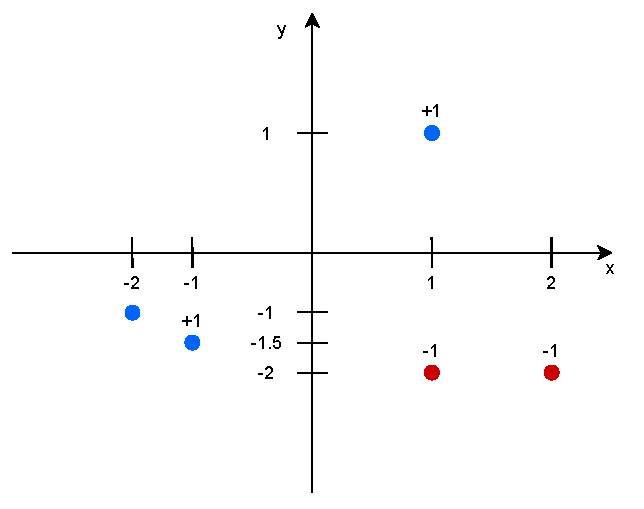
\includegraphics[scale = 0.8]{img/per1.pdf}
						\end{figure}
						Usiamo quindi l'algoritmo del percettrone e studiamo come si aggiornano i
						pesi. Si impone $\eta=0.2$ e nodo bias di valore $b=1$ e peso $w_0$,
						arbitrariamente inizializzato a 0.\\ 
						Partiamo con il primo esempio. Si hanno:
						\begin{itemize}
							\item $x_1=(1, 1)$
							\item $t(x_1)=1$
						\end{itemize}
						da ciò si ricava che l'input del percettrone, il suo segnale d'ingresso, altro
						non è che, considerando il nodo bias:
						\[\overline{x}=(b, x_1)=(1, 1, 1)\]
						Arbitrariamente inizializziamo i pesi a (avendo già detto che il bias ha peso
						0):
						\[\overline{w}=(0, 1, 0.5)\]
						Faccio quindi il prodotto scalare tra il vettore input e il vettore peso:
						\[\langle \overline{w}, \overline{x}\rangle=
							\left(\begin{matrix}
							0 & 1 & 0.5
							\end{matrix}\right)
							\left(
							\begin{matrix}
								1 \\
								1 \\
								1 \\
							\end{matrix}
							\right)= 0 + 1 + 0.5 = 1.5
						\]
						Si ha quindi $\langle \overline{w}, \overline{x}\rangle > 0$ e quindi:
						\[sign(\langle \overline{w}, \overline{x}\rangle)=+1\]
						e avendo che, ricordando $t(x_1)=+1$:
						\[sign(\langle \overline{w}, \overline{x}\rangle)=t(x_1)\]
						i pesi $\overline{w}$ non devono essere aggiornati.\\
						Si passa al secondo esempio.\\
						Si ha (senza dover rispiegare gli step metto tutto nella stessa lista):
						\begin{itemize}
							\item $x_2=(2,-2)$
							\item $t(x_2)=-1$
							\item $\overline{x}=(1, 2,-2)$
							\item $\overline{w}=(0, 1, 0.5)$
						\end{itemize}
						calcolo:
						\[\langle \overline{w}, \overline{x}\rangle=
							\left(\begin{matrix}
							0 & 1 & 0.5
							\end{matrix}\right)
							\left(
							\begin{matrix}
								1  \\
								2  \\
								-2 \\
							\end{matrix}
							\right)= 0 + 2 - 1 = 1
						\]
						Si ha quindi $\langle \overline{w}, \overline{x}\rangle > 0$ e quindi:
						\[sign(\langle \overline{w}, \overline{x}\rangle)=+1\]
						e avendo che, ricordando $t(x_2)=-1$:
						\[sign(\langle \overline{w}, \overline{x}\rangle)\neq t(x_2)\]
						Bisogna procedere all'update dei pesi, che ricordiamo essere:
						\[\overline{w}_{new}=\overline{w}_{old}+\eta(y-\hat{y})\overline{x}\]
						\newpage
						si ha quindi, avendo $\hat{y}=1, y=-1$ e quindi $y-\hat{y}=-2$:
						\begin{itemize}
							\item
							      $\overline{w}_{new}[0]=\overline{w}_{old}[0]+0.2\cdot (-2)\cdot
							      x[0]=0+0.2\cdot(-2)\cdot 1=-0.4$ 
							\item
							      $\overline{w}_{new}[1]=\overline{w}_{old}[1]+0.2\cdot (-2)\cdot
							      x[1]=1+0.2\cdot(-2)\cdot 2=0.2$ 
							\item
							      $\overline{w}_{new}[2]=\overline{w}_{old}[2]+0.2\cdot (-2)\cdot x[2]=0.5+0.2
							      \cdot(-2)\cdot(-2)=1.3$    
						\end{itemize}
						ottenendo quindi come nuovo vettore dei pesi:
						\[\overline{w}=(-0.4, 0.2, 1.3)\]
						Passo quindi al terzo esempio:
						\begin{itemize}
							\item $x_3=(-1,-1.5)$
							\item $t(x_3)=-1$
							\item $\overline{x}=(1,-1,-1.5)$
							\item $\overline{w}=(-0.4, 0.2, 1.3)$
						\end{itemize}
						calcolo:
						\[\langle \overline{w}, \overline{x}\rangle=
							\left(\begin{matrix}
							-0.4 & 0.2 & 1.3
							\end{matrix}\right)
							\left(
							\begin{matrix}
								1   \\
								-1  \\
								1.5 \\
							\end{matrix}
							\right)= -0.4-0.2-1.95 = -2.55
						\]
						Si ha quindi $\langle \overline{w}, \overline{x}\rangle \leq 0$ e quindi:
						\[sign(\langle \overline{w}, \overline{x}\rangle)=-1\]
						e avendo che, ricordando $t(x_3)=+1$:
						\[sign(\langle \overline{w}, \overline{x}\rangle)\neq t(x_3)\]
						Bisogna procedere all'update dei pesi, avendo $\hat{y}=-1, y=1$ e quindi
						$y-\hat{y}=2$:
						\begin{itemize}
							\item
							      $\overline{w}_{new}[0]=\overline{w}_{old}[0]+0.2\cdot 2\cdot
							      x[0]=-0.4+0.2\cdot 2\cdot 1=0$ 
							\item
							      $\overline{w}_{new}[1]=\overline{w}_{old}[1]+0.2\cdot 2\cdot
							      x[1]=0.2+0.2\cdot 2\cdot (-1)=-0.2$ 
							\item
							      $\overline{w}_{new}[2]=\overline{w}_{old}[2]+0.2\cdot 2\cdot x[2]=1.3+0.2
							      \cdot 2\cdot(-1.5)=0.7$    
						\end{itemize}
						ottenendo quindi come nuovo vettore dei pesi:
						\[\overline{w}=(0, -0.2, 0.7)\]
						Passo quindi al quarto esempio:
						\begin{itemize}
							\item $x_4=(1,-2)$
							\item $t(x_4)=-1$
							\item $\overline{x}=(1, 1,-2)$
							\item $\overline{w}=(0, -0.2, 0.7)$
						\end{itemize}
						calcolo:
						\[\langle \overline{w}, \overline{x}\rangle=
							\left(\begin{matrix}
							0 & -0.2 & 0.7
							\end{matrix}\right)
							\left(
							\begin{matrix}
								1  \\
								1  \\
								-2 \\
							\end{matrix}
							\right)= 0-0.2-1.4 = -1.6
						\]
						Si ha quindi $\langle \overline{w}, \overline{x}\rangle \leq 0$ e quindi:
						\[sign(\langle \overline{w}, \overline{x}\rangle)=-1\]
						e avendo che, ricordando $t(x_4)=-1$:
						\[sign(\langle \overline{w}, \overline{x}\rangle)= t(x_4)\]
						E quindi non devo aggiornare i pesi.\\
						Passo quindi al quinto esempio:
						\begin{itemize}
							\item $x_5=(-2,-1)$
							\item $t(x_5)=1$
							\item $\overline{x}=(1,-2,-1)$
							\item $\overline{w}=(0, -0.2, 0.7)$
						\end{itemize}
						calcolo:
						\[\langle \overline{w}, \overline{x}\rangle=
							\left(\begin{matrix}
							0 & -0.2 & 0.7
							\end{matrix}\right)
							\left(
							\begin{matrix}
								1  \\
								-2 \\
								-1 \\
							\end{matrix}
							\right)= 0+0.4-0.7 = -0.3
						\]
						Si ha quindi $\langle \overline{w}, \overline{x}\rangle \leq 0$ e quindi:
						\[sign(\langle \overline{w}, \overline{x}\rangle)=-1\]
						e avendo che, ricordando $t(x_5)=+1$:
						\[sign(\langle \overline{w}, \overline{x}\rangle)\neq t(x_5)\]
						Bisogna procedere all'update dei pesi, avendo $\hat{y}=-1, y=1$ e quindi
						$y-\hat{y}=2$:
						\begin{itemize}
							\item
							      $\overline{w}_{new}[0]=\overline{w}_{old}[0]+0.2\cdot 2\cdot
							      x[0]=0+0.2\cdot 2\cdot 1=0.4$ 
							\item
							      $\overline{w}_{new}[1]=\overline{w}_{old}[1]+0.2\cdot 2\cdot
							      x[1]=0.2+0.2\cdot 2\cdot (-2)=-1$ 
							\item
							      $\overline{w}_{new}[2]=\overline{w}_{old}[2]+0.2\cdot 2\cdot x[2]=0.7+0.2
							      \cdot 2\cdot(-1)=0.3$    
						\end{itemize}
						ottenendo quindi come nuovo vettore dei pesi:
						\[\overline{w}=(0.4, -1, 0.3)\]
						che, avendo terminato l'esercizio, è il vettore pesi finale usato
						dall'algoritmo. 
					\end{esercizio}
					\subsection{Reti multistrato}
					\textbf{Le formule più complesse sono solo di bellezza.}\\
					\noindent
					Passiamo quindi dal percettrone a una rete a due strati, cambiando quindi la
					gestione dei pesi.\\
					Devo avere sempre un gradiente dei pesi, che ora avranno doppio indice per
					indicare anche l'unità di riferimento, che scende:
					\[\frac{\partial E}{\partial w_{ij}}=\frac{\partial E}{\partial y_{j}}\cdot
						\frac{\partial y_j}{\partial w_{ij}}=-(t_j-y_j)\cdot \frac{\partial
							y_j}{\partial w_{ij}}=-\delta_j\cdot\frac{\partial \sum_i w_{ij}\cdot
							x_j}{\partial w_{ij}}=-\delta_j\cdot x_i\]
						Si ha quindi:
						\[\Delta w_{ij}=\eta\cdot \delta_j\cdot x_i\]
						detta \textbf{regola delta}, che è l'evoluzione di quanto detto per il
						percettrone in merito alla variazione dei pesi.\\
						Si ha che la convergenza a un minimo globale é garantita per funzioni di
						attivazione lineari senza unità nascoste e per dati consistenti.\\
						Si introduce una nuova funzione di attivazione, detta \textbf{sigmoide}, che
						comporta l'\textbf{unità sigmoide}. La funzione sigmoide è:
						\[y=\sigma(net)=\frac{1}{1+e^{-net}}\]
						Tale funzione è derivabile, infatti:
						\[\dd \sigma(x)=\sigma(x)\cdot (1-\sigma(x))\]
						riprendendo la figura \ref{fig:bin} si ha quindi in primis l'aggiunta del nodo
						bias e poi il cambio della funzione a scalino con il \textbf{sigmoide}. L'output
						invece non sarà più binario ma un certo $y$.\\
						Si hanno quindi in primis le \textbf{reti multistrato feedforward} con le
						seguenti caratteristiche:
						\begin{itemize}
							\item si hanno strati intermedi tra input e output
							\item si hanno connessioni da strati di livello basso a strati di livello
							      alto, solitamente mono direzionali
							\item non si hanno all'interno di uno stesso strato
							\item il neurone ha uno stato booleano $x\in\{0, 1\}$
							\item si ha la seguente funzione di transizione:
							      \[x_k=\sigma\left(\sum_{j}w_{jk}\cdot x_j\right)\]
							      con $x_j$ che può essere in alcuni
							      casi un input istanza e in altri lo stato di altri neuroni, a seconda
							      dell'altezza del livello in cui mi trovo
							\item per ogni configurazione $x$ del primo strato (ingresso), la rete calcola
							      una configurazione $y$ dell'ultimo strato (uscita). Normalmente avremo uno
							      strato nascosto più grande (poco) di quello d'uscita (anche se non si ha una
							      regola per dimensionare lo strato nascosto). Raramente useremo più strati
							      nascosti
						\end{itemize}
						\begin{figure}
							\centering
							\psscalebox{0.8 0.8} % Change this value to rescale the drawing.
							{
								\begin{pspicture}(-3,-4.18)(7.52, 4.18)
									\definecolor{colour2}{rgb}{0.96862745, 0.3019608, 0.3019608}
									\definecolor{colour1}{rgb}{0.003921569, 0.003921569, 0.003921569}
									\definecolor{colour3}{rgb}{0.039215688, 0.5647059, 0.1882353}
									\definecolor{colour4}{rgb}{0.078431375, 0.28627452, 0.8784314}
									\pscircle[linecolor=black, linewidth=0.04, dimen=outer]
									(2.4, 2.7049024){0.4}
									\pscircle[linecolor=black, linewidth=0.04, dimen=outer]
									(2.4, 0.70490235){0.4}
									\pscircle[linecolor=black, linewidth=0.04, dimen=outer]
									(4.0, 0.70490235){0.4}
									\pscircle[linecolor=black, linewidth=0.04, dimen=outer]
									(0.8, 0.70490235){0.4}
									\pscircle[linecolor=black, linewidth=0.04, dimen=outer]
									(2.4,-0.8950977){0.4}
									\pscircle[linecolor=black, linewidth=0.04, dimen=outer]
									(4.0,-0.8950977){0.4}
									\pscircle[linecolor=black, linewidth=0.04, dimen=outer]
									(0.8,-0.8950977){0.4}
									\pscircle[linecolor=black, linewidth=0.04, dimen=outer]
									(1.6,-2.8950977){0.4}
									\pscircle[linecolor=black, linewidth=0.04, dimen=outer]
									(3.2,-2.8950977){0.4}
									\psline[linecolor=black, linewidth=0.04, arrowsize=0.05291667cm 2.0,
									arrowlength=1.4, arrowinset=0.0]{<-}(2.4, 2.3049023)(0.8, 1.1049024)
									\psline[linecolor=black, linewidth=0.04, arrowsize=0.05291667cm 2.0,
									arrowlength=1.4, arrowinset=0.0]{<-}(2.4, 2.3049023)(2.4, 1.1049024)
									\psline[linecolor=black, linewidth=0.04, arrowsize=0.05291667cm 2.0,
									arrowlength=1.4, arrowinset=0.0]{<-}(2.4, 2.3049023)(4.0, 1.1049024)
									\psline[linecolor=black, linewidth=0.04, arrowsize=0.05291667cm 2.0,
									arrowlength=1.4, arrowinset=0.0]{<-}(0.8,-1.2950977)(1.6,-2.4950976)
									\psline[linecolor=black, linewidth=0.04, arrowsize=0.05291667cm 2.0,
									arrowlength=1.4, arrowinset=0.0]{<-}(0.8,-1.2950977)(3.2,-2.4950976)
									\psline[linecolor=black, linewidth=0.04, arrowsize=0.05291667cm 2.0,
									arrowlength=1.4, arrowinset=0.0]{<-}(2.4,-1.2950977)(1.6,-2.4950976)
									\psline[linecolor=black, linewidth=0.04, arrowsize=0.05291667cm 2.0,
									arrowlength=1.4, arrowinset=0.0]{<-}(2.4,-1.2950977)(3.2,-2.4950976)
									\psline[linecolor=black, linewidth=0.04, arrowsize=0.05291667cm 2.0,
									arrowlength=1.4, arrowinset=0.0]{<-}(4.0,-1.2950977)(3.2,-2.4950976)
									\psline[linecolor=black, linewidth=0.04, arrowsize=0.05291667cm 2.0,
									arrowlength=1.4, arrowinset=0.0]{<-}(4.0,-1.2950977)(1.6,-2.4950976)
									\psdots[linecolor=black, dotsize=0.04](1.2,-0.09509765)
									\psdots[linecolor=black, dotsize=0.04](1.6,-0.09509765)
									\psdots[linecolor=black, dotsize=0.04](2.0,-0.09509765)
									\psdots[linecolor=black, dotsize=0.04](2.8,-0.09509765)
									\psdots[linecolor=black, dotsize=0.04](3.2,-0.09509765)
									\psdots[linecolor=black, dotsize=0.04](3.6,-0.09509765)
									\psframe[linecolor=colour2, linewidth=0.04, dimen=outer]
									(4.4,-2.0950975)(0.4,-3.6950977)
									\rput[bl](1.2,-4.0950975){\textcolor{colour1}{strato d'input}}
									\rput[bl](1, 3.6049025){\textcolor{colour1}{strato di output}}
									\rput[bl](5,-0.19509765){\textcolor{colour1}{strati nascosti}}
									\psframe[linecolor=colour3, linewidth=0.04, dimen=outer]
									(4.0, 3.5049024)(0.8, 1.9049023)
									\psframe[linecolor=colour4, linewidth=0.04, dimen=outer]
									(4.8, 1.5049024)(0.0,-1.6950977)
								\end{pspicture}
							}
							\caption{Rappresentazione stilizzata di rete multistrato}
						\end{figure}
						Quindi fissata una mappa $f$ tra input e output, sulla base degli stimoli $x_i$,
						la rete cambia i pesi in modo che dopo un numero di passi $s$ si abbia l'output
						$y_k$ tale che $f(x_k)=y_k,\forall\, k>s$ (almeno approssimativamente). Per la
						modifica bisogna minimizzare un c\textbf{riterio di discrepanza} tra risposta
						della rete e risposta desiderata.\\
						In questo modo potremmo anche risolvere il problema dell'\textit{or esclusivo},
						aggiungendo uno strato nascosto.\\
						Viene aumentata la potenza rispetto al percettrone, permettendo una
						classificazione \textbf{altamente non lineare}.\\
						Si hanno quindi $u_1,\ldots, u_n$ neuroni divisi in:
						\begin{itemize}
							\item unità d'input
							\item unità nascoste
							\item unità di output
						\end{itemize}
						Si hanno inoltre:
						\begin{itemize}
							\item pesi $w_jj$ per ogni coppia che voglio connettere
							\item stati di attivazione $s_j\in \mathbb{R}$
							\item input netto a $u_j$: $n_i=\sum_{i=0}^n w_{ij}\cdot s_i$
							\item funzione di transizione sigmoide:
							      \[s_j(t+1)=\frac{1}{1+e^{-n_i(t)}}\]
						\end{itemize}
						Lo stato di uscita è determinato da una serie di strati profondi. Dato un input
						$x$, un output target $t$ e un output effettivo $y$ abbiamo la solita forma
						quadratica:
						\[E=\frac{1}{2}\sum_j(t_j-y_j)^2\]
						che dipende anche dagli strati nascosti. In ogni caso si ha:
						\[\Delta w_{ij}=-\eta\cdot\frac{\partial E}{\partial w_{ij}}\]
						poiché:
						\[\frac{\partial E}{\partial w_{ij}}= \frac{\partial E}{\partial n_{j}}\cdot
							\frac{\partial n_j}{\partial w_{ij}}= \frac{\partial E}{\partial n_{j}}\cdot
							s_j=(def)-\delta_j\cdot s_j\]
							e si cerca:
							\[\delta_j=-\frac{\partial E}{\partial n_{j}}\]
							Abbiamo quindi l'\textbf{algoritmo di retropropagazione} che si divide in 5
							passi:
							\begin{enumerate}
								\item \textbf{input}: al neurone d'input $u_j$ viene assegnato lo stato $x_j$
								        
								\item \textbf{propagazione}: si calcola lo stato dei neuroni nascosti o di
								      output $u_j$:
								      \[s_j=f_j(n_j)\]
								\item \textbf{confronto}: per ogni neurone di output $u_j$, noto l’output
								      atteso $t_j$, si calcola:
								      \[\delta_j=f_j(n_j)\cdot(t_j-y_j))\]
								\item \textbf{retropropagazione dell’errore}: per ogni neurone nascosto $u_j$,
								      si calcola:
								      \[\delta_j=f_j(n_j)\cdot\left(\sum_h w_{ih}\cdot \delta_h\right)\]
								\item \textbf{aggiornamento dei pesi}: si ha:
								      \[w_{ij}=w_{ij}+\eta\cdot \delta_i\cdot s_j\]
							\end{enumerate}
							Vediamo quindi l'algoritmo:
							\begin{algorithm}[H]
								\begin{algorithmic}
									\Function{ret-prog}{}
									\State \textit{inizializzo ogni $\Delta w_i$ a un valore piccolo casuale}
									\While {\textit{non raggiungimento della condizione di terminazione}}
									\For {\textit{ogni esempio $\langle (x_1,\ldots, x_n), t\rangle$}}
									\State \textit{immetto l'input $( x_1, \ldots x_n)$ nella rete e calcolo
									$y_k$}  
									\For {\textit{ogni unità di output $k$}}
									\[\delta_k=y_k\cdot(1-y_k)\cdot(t_k-y_k)\]
									\EndFor
									\For {\textit{ogni unità nascosta $h$}}
									\[\delta_h=y_h\cdot(1-y_h)\cdot\sum_k w_{hk}\delta_k\]
									\EndFor
									\For {\textit{ogni peso $w_{ij}$}}
									\[w_{ij}=w_{ij}+\Delta w_{ij},\mbox{con } \Delta w_{ij}=\eta\cdot\delta_j\cdot x_{ij}\] 
									\EndFor
									\EndFor
									\EndWhile
									\State \textit{aggiorno i pesi:}
									\[w_i=w_i+\Delta w_i\]
									\EndFunction
								\end{algorithmic}
								\caption{Algoritmo di retropropagazione}
							\end{algorithm}
							Questa tecnica si generalizza facilmente a grafi orientati.\\  
							Si trova però un \textbf{minimo locale} e non \textbf{globale} e spesso
							include \textbf{termini di momento} per cambiare la formula dell'aggiornamento
							dei pesi del tipo: 
							\[\Delta w_{ij}(n)=\eta\cdot \delta_j\cdot x_{ij}+\alpha\Delta w_{ij}(n-1)\]
							in modo da avere una sorta di \textit{inerzia} per la variazione dei pesi.\\
							Ci sono comunque modelli per uscire dai minimi locali (usando alcune tecniche di
							\textit{ricerca operativa}).\\
							Si minimizzano gli errori sugli esempi di training m, a si rischia
							l'\textbf{overfitting}.\\
							Tutti questi fattori comportano un addestramento lento ma dopo l'addestramento
							si ha una rete veloce.\\
							Si hanno quindi i seguenti limiti:
							\begin{itemize}
								\item mancanza di teoremi generali di convergenza
								\item può portare in minimi locali di $E$ 
								\item difficoltà per la scelta dei parametri 
								\item scarsa capacità di generalizzazione 
							\end{itemize}
							Si possono avere varianti al modello tramite:
							\begin{itemize}
								\item un tasso di apprendimento adattivo:
								      \[\eta=g(\nabla E)\]
								\item range degli stati da –1 a 1 
								\item l'uso di \textit{termini di momento}
								\item deviazioni dalla discesa più ripida 
								\item variazioni nell'architettura (numero di strati nascosti)
								\item inserimento di connessioni all'indietro
							\end{itemize}
							\textit{Le reti \textbf{feedforward} sono state usate in progetti di guida
								autonoma come \textbf{ALVINN}.}\\
							Rispetto alberi decisionali si ha:
							\begin{itemize}
								\item le reti neurali sono più lente in fase di apprendimento ma uguali in
								      fase di esecuzione
								\item le reti neurali hanno una migliore tolleranza del rumore
								\item le reti neurali sono meno conoscibili dopo l'esecuzione
								\item miglior accuratezza (?)
							\end{itemize}
							Si nota che ne le reti neurali ne gli alberi decisionali possono usare della
							conoscenza a priori.
							\subsubsection{Esercitazione reti neurali multistrato}
							\begin{esercizio}
								vengono date le istanze:
								\[z_1=(0, 2, 2)\]
								\[z_2=1, 0, 0\]
								Con la seguente architettura:
								\begin{figure}[H]
									\centering
									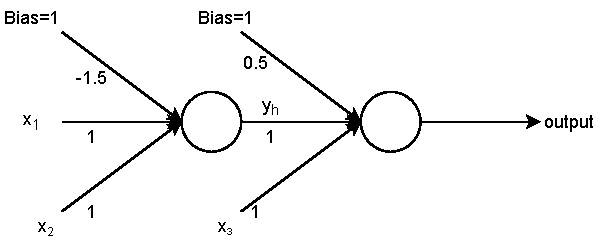
\includegraphics[scale = 0.9]{img/per2.pdf}
								\end{figure}
								con quindi una terza istanza valutata solo nel secondo livello.\\
								La funzione $f$ di attivazione del neurone è definita come quella del
								percettrone, ovvero:
								\[sgn(x)=
									\begin{cases}
										1  & \mbox{se } x\geq 0 \\
										-1 & \mbox{altrimenti}  
									\end{cases}
								\]
								L'esercizio propone di capire la label assegnata a $z_1$ e la label assegnata
								a $z_2$.\\
								Nel dettaglio, per entrambe le istanze, abbiamo $(x_1, x_2, x_3)$, ovvero i
								primi due valori sono (insieme al bias) l'input del primo layer mentre il
								terzo (insieme al bias e al risultato del primo layer) è l'input del secondo
								layer.\\
								Partiamo con $x_1=(0, 2, 2)$.\\
								Si hanno i due layer:
								\begin{enumerate}
									\item nel layer 1 si ha:
									      \[\langle \overline{x},\overline{w}\rangle=
									      	\left(\begin{matrix}
									      	1 & 0 & 2
									      	\end{matrix}\right)
									      	\left(
									      	\begin{matrix}
									      		-1.5 \\
									      		1    \\
									      		1    \\
									      	\end{matrix}
									      	\right)= -1.5+0+2 = 0.5\]
									      	Si ha quindi:
									      	\[\langle \overline{x},\overline{w}\rangle\geq 0\]
									      	e quindi:
									      	\[sgn(\langle \overline{x},\overline{w}\rangle)=sgn(0.5)=1\]
									      	avendo quindi:
									      	\[y_h=1\]
									      	che sarà tra gli input del secondo layer
									      	\item valuto quindi il layer 2:
									      	\[\langle \overline{x},\overline{w}\rangle=
									      		\left(\begin{matrix}
									      		1 & 1 & 2
									      		\end{matrix}\right)
									      		\left(
									      		\begin{matrix}
									      			-0.5 \\
									      			1    \\
									      			1    \\
									      		\end{matrix}
									      		\right)= -0.5+1+2 = 2.5\]
									      		Si ha quindi:
									      		\[\langle \overline{x},\overline{w}\rangle\geq 0\]
									      		e quindi:
									      		\[sgn(\langle \overline{x},\overline{w}\rangle)=sgn(2.5)=1\]
									      		avendo quindi:
									      		\[output=1\]
									      		\end{enumerate}
									      		Possiamo quindi dire che per la prima istanza:
									      		\[f(x_1)=+1\]
									      		Passiamo a $x_2=(1, 0, 0)$.\\
									      		Si hanno i due layer:
									      		\begin{enumerate}
									      			\item nel layer 1 si ha:
									      			      \[\langle \overline{x},\overline{w}\rangle=
									      			      	\left(\begin{matrix}
									      			      	1 & 1 & 0
									      			      	\end{matrix}\right)
									      			      	\left(
									      			      	\begin{matrix}
									      			      		-1.5 \\
									      			      		1    \\
									      			      		1    \\
									      			      	\end{matrix}
									      			      	\right)= -1.5+1+0 = -0.5\]
									      			      	Si ha quindi:
									      			      	\[\langle \overline{x},\overline{w}\rangle< 0\]
									      			      	e quindi:
									      			      	\[sgn(\langle \overline{x},\overline{w}\rangle)=sgn(-0.5)=-1\]
									      			      	avendo quindi:
									      			      	\[y_h=-1\]
									      			      	che sarà tra gli input del secondo layer
									      			      	\item valuto quindi il layer 2:
									      			      	\[\langle \overline{x},\overline{w}\rangle=
									      			      		\left(\begin{matrix}
									      			      		1 & -1 & 0
									      			      		\end{matrix}\right)
									      			      		\left(
									      			      		\begin{matrix}
									      			      			-0.5 \\
									      			      			1    \\
									      			      			1    \\
									      			      		\end{matrix}
									      			      		\right)= -0.5-1+0 = -1.5\]
									      			      		Si ha quindi:
									      			      		\[\langle \overline{x},\overline{w}\rangle < 0\]
									      			      		e quindi:
									      			      		\[sgn(\langle \overline{x},\overline{w}\rangle)=sgn(-1.5)=-1\]
									      			      		avendo quindi:
									      			      		\[output=-1\]
									      			      		\end{enumerate}
									      			      		Possiamo quindi dire che per la prima istanza:
									      			      		\[f(x_2)=-1\]
									      			      		Abbiamo quindi classificato la prima istanza come positiva e la seconda come
									      			      		negativa.
									      			      		\begin{shaded}
									      			      			\textbf{Ripasso di algebra lineare}\\
									      			      			Per praticità ripasseremo i concetti fondamentali facendo riferimento a
									      			      			$\mathbb{R}^2$, formato quindi da elementi, dette coordinate, che sono coppie
									      			      			ordinate $(x_1, x_2)$ (rappresentabili con un punto nel piano o con un segmento
									      			      			orientato con partenza nell'origine e destinazione nelle coordinate del punto
									      			      			nel piano).\\
									      			      			Ricordiamo le operazioni fondamentali, dati $R$ pari a $(x_1, x_2)$ e $Q$ pari
									      			      			a $(x_3, x_4)$ 
									      			      			\begin{itemize}
									      			      				\item addizione: $P+Q=(x_1+x_3, x_2+x_4)$
									      			      				\item prodotto per uno scalare $\lambda\in\mathbb{R}$: $\lambda\cdot
									      			      				      R=(\lambda\cdot x_1,\lambda\cdot x_2)$
									      			      				\item prodotto scalare tra vettori: $\langle P, Q\rangle\equiv P\cdot Q^T =
									      			      				      \sum_{i=1}^n r_i\cdot q_i$ 
									      			      				      (dove $r_i$ e $q_i$ sono rispettivamente gli elementi di $R$ e $Q$
									      			      				      all'indice $i$)
									      			      			\end{itemize}
									      			      			Ricordiamo la \textit{norma} di un vettore $X$:
									      			      			\[\norm{X}=\equiv\sqrt{X\cdot X^T}=\sqrt{\sum_{i=1}^n x_i\cdot
									      			      					x_i}=\sqrt{\langle X, X\rangle}\] 
									      			      				Con $X=0$ indichiamo il \textit{vettore nullo} (che ha anche norma nulla).\\
									      			      				Definiamo il \textit{versore} (\textit{vettore unitario}) come:
									      			      				\[\frac{X}{\norm{X}},\,\,\, X\neq 0\]
									      			      				In $\mathbb{R}^2$ l'angolo $\theta$ sotteso tra due vettori $X$ e $Y$ è:
									      			      				\[\cos\theta=\frac{\langle X, Y\rangle}{\norm{X}\cdot \norm{Y}}\]
									      			      				La proiezione di un vettore $X$ sul vettore $Y$ è:
									      			      				\[X_Y=\norm{X}\cdot \cos\theta\]
									      			      				Si hanno quindi tre casi:
									      			      				\begin{enumerate}
									      			      					\item $\theta < 90 \iff \langle X, Y\rangle >0$
									      			      					\item $\theta > 90 \iff \langle X, Y\rangle <0$
									      			      					\item $\theta = 90 \iff \langle X, Y\rangle =0$
									      			      				\end{enumerate}
									      			      				(quindi disegnando una retta sul piano tutti i punti sopra di essa
									      			      				apparterranno a una certa classe e quelli sotto a un'altra).\\
									      			      				Posso definire una retta $r$ che passa per l'origine in  $\mathbb{R}^2$
									      			      				assegnando un vettore $W=(w_1, w_2)$ ad essa ortogonale, infatti tutti i punti,
									      			      				ovvero vettori, $X=(x_1, x_2)$ sulla retta sono ortogonali a $W$:
									      			      				\[\langle W, X\rangle=w_1\cdot x_1+w_2\cdot x_2=0 \]
									      			      				Quindi la retta (ovvero l'iperpiano) mi separa due semispazi, a seconda che
									      			      				$\langle X, W\rangle$ sia strettamente positivo o strettamente negativo.\\
									      			      				Generalizzando ora a $n$ dimensioni ho che, dato l'iperpiano $h$ (di
									      			      				dimensione $n-1$):
									      			      				\begin{itemize}
									      			      					\item se $h$ passa dall'origine allora si ha l'equazione $\langle X, Y\rangle
									      			      					      =0$
									      			      					\item se non passa per l'origine $\langle X, Y\rangle +b=0$ 
									      			      					          
									      			      				\end{itemize}
									      			      				I vettori in un iperpiano si proiettano tutti nello stesso modo e i punti ad
									      			      				un lato e all'altro dell'iperpiano sono distinti dal fatto che $\langle
									      			      				X, Y\rangle +b$ sia strettamente positiva o strettamente negativa
									      			      				\end{shaded}
									      			      				\end{esercizio}